% !TEX TS-program = pdflatex
% !TEX encoding = UTF-8 Unicode

% This file is a template using the "beamer" package to create slides for a talk or presentation
% - Giving a talk on some subject.
% - The talk is between 15min and 45min long.
% - Style is ornate.

% MODIFIED by Jonathan Kew, 2008-07-06
% The header comments and encoding in this file were modified for inclusion with TeXworks.
% The content is otherwise unchanged from the original distributed with the beamer package.

\documentclass{beamer}


% Copyright 2004 by Till Tantau <tantau@users.sourceforge.net>.
%
% In principle, this file can be redistributed and/or modified under
% the terms of the GNU Public License, version 2.
%
% However, this file is supposed to be a template to be modified
% for your own needs. For this reason, if you use this file as a
% template and not specifically distribute it as part of a another
% package/program, I grant the extra permission to freely copy and
% modify this file as you see fit and even to delete this copyright
% notice. 


\mode<presentation>
{
  \usetheme{default}
  % or ...

  \setbeamercovered{transparent}
  % or whatever (possibly just delete it)
}


\usepackage[english]{babel}
% or whatever

\usepackage[utf8]{inputenc}
% or whatever

\usepackage{times}
\usepackage[T1]{fontenc}
%\RequirePackage[numbers,sort&compress,square,comma]{natbib}
%\bibliographystyle{IEEEtranN}
% Or whatever. Note that the encoding and the font should match. If T1
% does not look nice, try deleting the line with the fontenc.

\usepackage[authoryear,round,colon]{natbib}
\bibliographystyle{plainnat}
\def\newblock{\hskip .11em plus .33em minus .07em}

\title[Parallel Graph Reduction] % (optional, use only with long paper titles)
{Parallel Graph Reduction for Implementing Functional Languages}

\subtitle
{} % (optional)

\author[] % (optional, use only with lots of authors)
{J. M. Calder\'{o}n Trilla}
% - Use the \inst{?} command only if the authors have different
%   affiliation.

\institute[University of York] % (optional, but mostly needed)
{%
  Department of Computer Science\\
  PLASMA Research Group \\
  University of York
 }
% - Use the \inst command only if there are several affiliations.
% - Keep it simple, no one is interested in your street address.

\date[] % (optional)
{19-01-2012 / Literature Review Seminar}

\subject{Talks}
% This is only inserted into the PDF information catalog. Can be left
% out. 



% If you have a file called "university-logo-filename.xxx", where xxx
% is a graphic format that can be processed by latex or pdflatex,
% resp., then you can add a logo as follows:

% \pgfdeclareimage[height=0.5cm]{university-logo}{university-logo-filename}
% \logo{\pgfuseimage{university-logo}}



% Delete this, if you do not want the table of contents to pop up at
% the beginning of each subsection:
\AtBeginSubsection[]
{
  \begin{frame}<beamer>{Outline}
    \tableofcontents[currentsection,currentsubsection]
  \end{frame}
}


% If you wish to uncover everything in a step-wise fashion, uncomment
% the following command: 

%\beamerdefaultoverlayspecification{<+->}


\begin{document}

\begin{frame}
  \titlepage
\end{frame}

\begin{frame}{Outline}
  \tableofcontents
  % You might wish to add the option [pausesections]
\end{frame}


% Since this a solution template for a generic talk, very little can
% be said about how it should be structured. However, the talk length
% of between 15min and 45min and the theme suggest that you stick to
% the following rules:  

% - Exactly two or three sections (other than the summary).
% - At *most* three subsections per section.
% - Talk about 30s to 2min per frame. So there should be between about
%   15 and 30 frames, all told.

\section{Introduction}

\subsection[Motivation]{Motivation}

\begin{frame}{Motivation for Parallel Functional Language Implementations}
    \begin{itemize}
        \item
            Parallel programming in imperative style is difficult. The lack of state in
            functional programs provides an advantage \citep{PFPAnIntro}.
\pause
        \item
            The largest successes in large scale parallelism have come from the declarative
            and functional paradigms (Databases, Map/Reduce).
    \end{itemize}
\end{frame}

\begin{frame}{Moore's Law's Effect on Parallel Functional Programming}
    \begin{itemize}
        \item
            Throughout the 80's researchers worked on parallel graph reduction for functional
            programs. However, the research could not keep up with the massive increase
            in single CPU processing speed/power. 
\pause
        \item
            Moore's law is still holding, but single thread CPUs are not seeing the same speed
            increases. Additional power is continually coming from increasing the number of 
            processing cores.
             
    \end{itemize}
\end{frame}

\subsection{Conference Publications for PFP from 1980-2011}

\begin{frame}[fragile]{Publication counts for Parallel Functional Programming}{}
    \begin{figure}
    \centering
        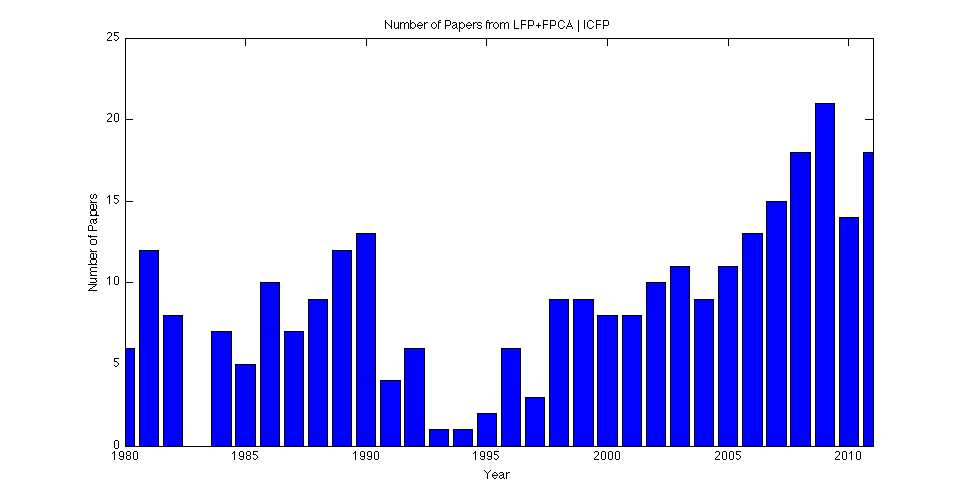
\includegraphics[scale=.4]{figures/numPapers.png}
        \caption{The ebb and flow of PFP}
    \end{figure}

\end{frame}

\section{Abstract Machines}
\subsection[Design Choices for Parallel Implementations of Functional Languages]{Design Choices for Parallel Implementations of FL}

\begin{frame}{Abstract Machines: Design Choices \citep{clackBook}}
    \begin{enumerate}
        \item Graph can be stored centrally, or distributed amongst several memories;
\pause
        \item Each processing agent is made up of \emph{one or more} sequential abstract
                machines that execute a thread;
\pause
        \item Threads that are not being executed reside in one or more thread pools, threads
                that have not begun evaluation are known as sparks;
\pause
        \item Synchronization is required between processing agents when the result of a reduction
                is needed by another thread 
    \end{enumerate}
\end{frame}

\subsection[The $< \nu, G> Machine$]{The $< \nu, G> Machine$}

\begin{frame}{Simple G-Machine}
Stack based machine with `G-Code' used as an intermediate language. G-Code is generated for
every supercombinator in the program, leaving the G-Machine with a set of G-Code fragments.  
    \begin{figure}
    \centering
        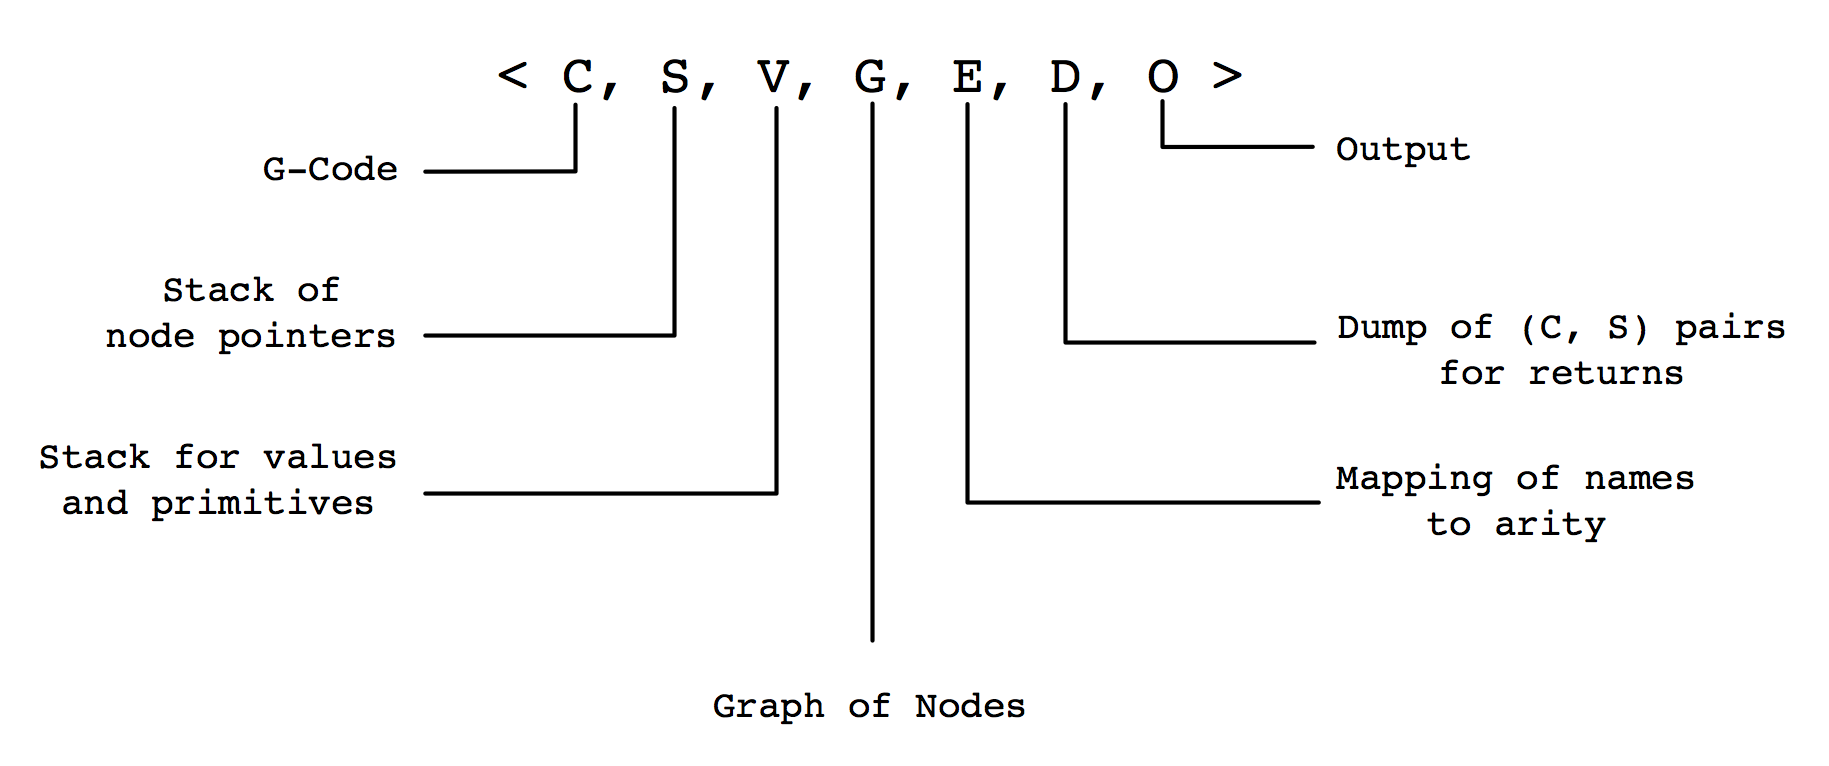
\includegraphics[scale=.3]{figures/GMachineState.png}
    \end{figure}
\end{frame}

\begin{frame}{Example Graph Reduction}
    \begin{figure}
    \centering
        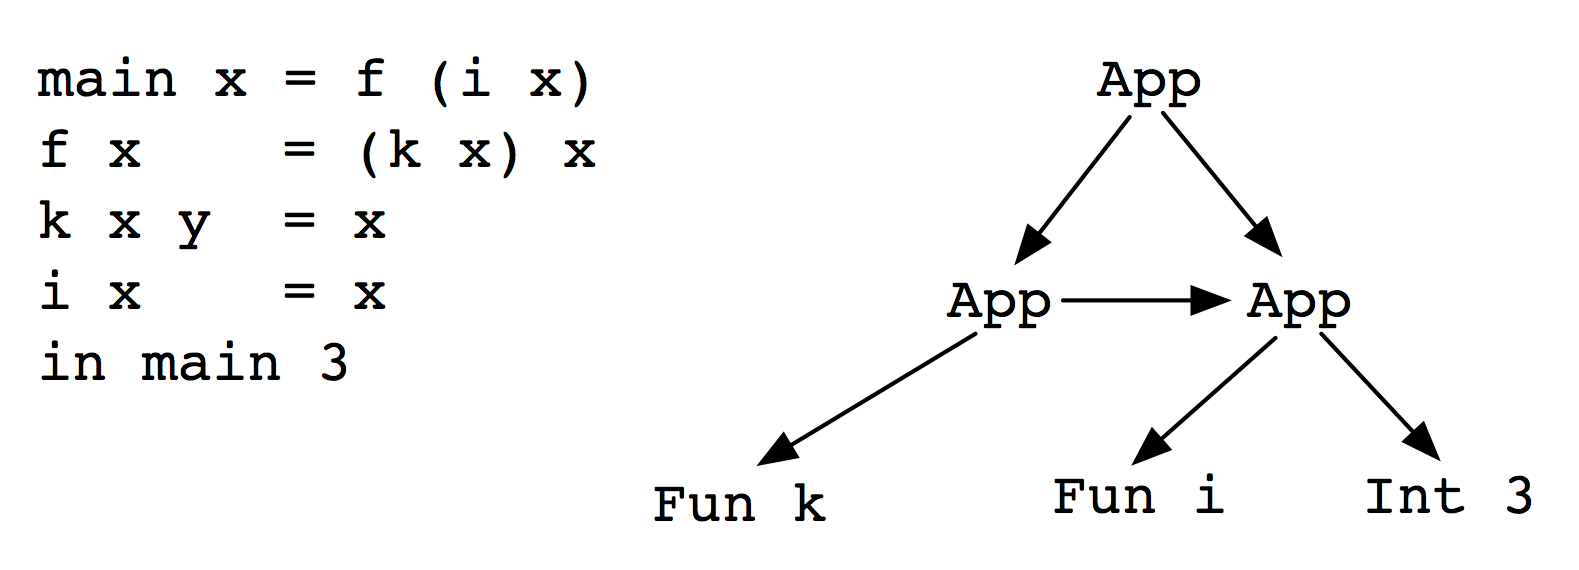
\includegraphics[scale=.3]{figures/GraphRed1.png}
    \end{figure}
\end{frame}

\begin{frame}{Simple Parallelization}
    \begin{figure}
    \centering
        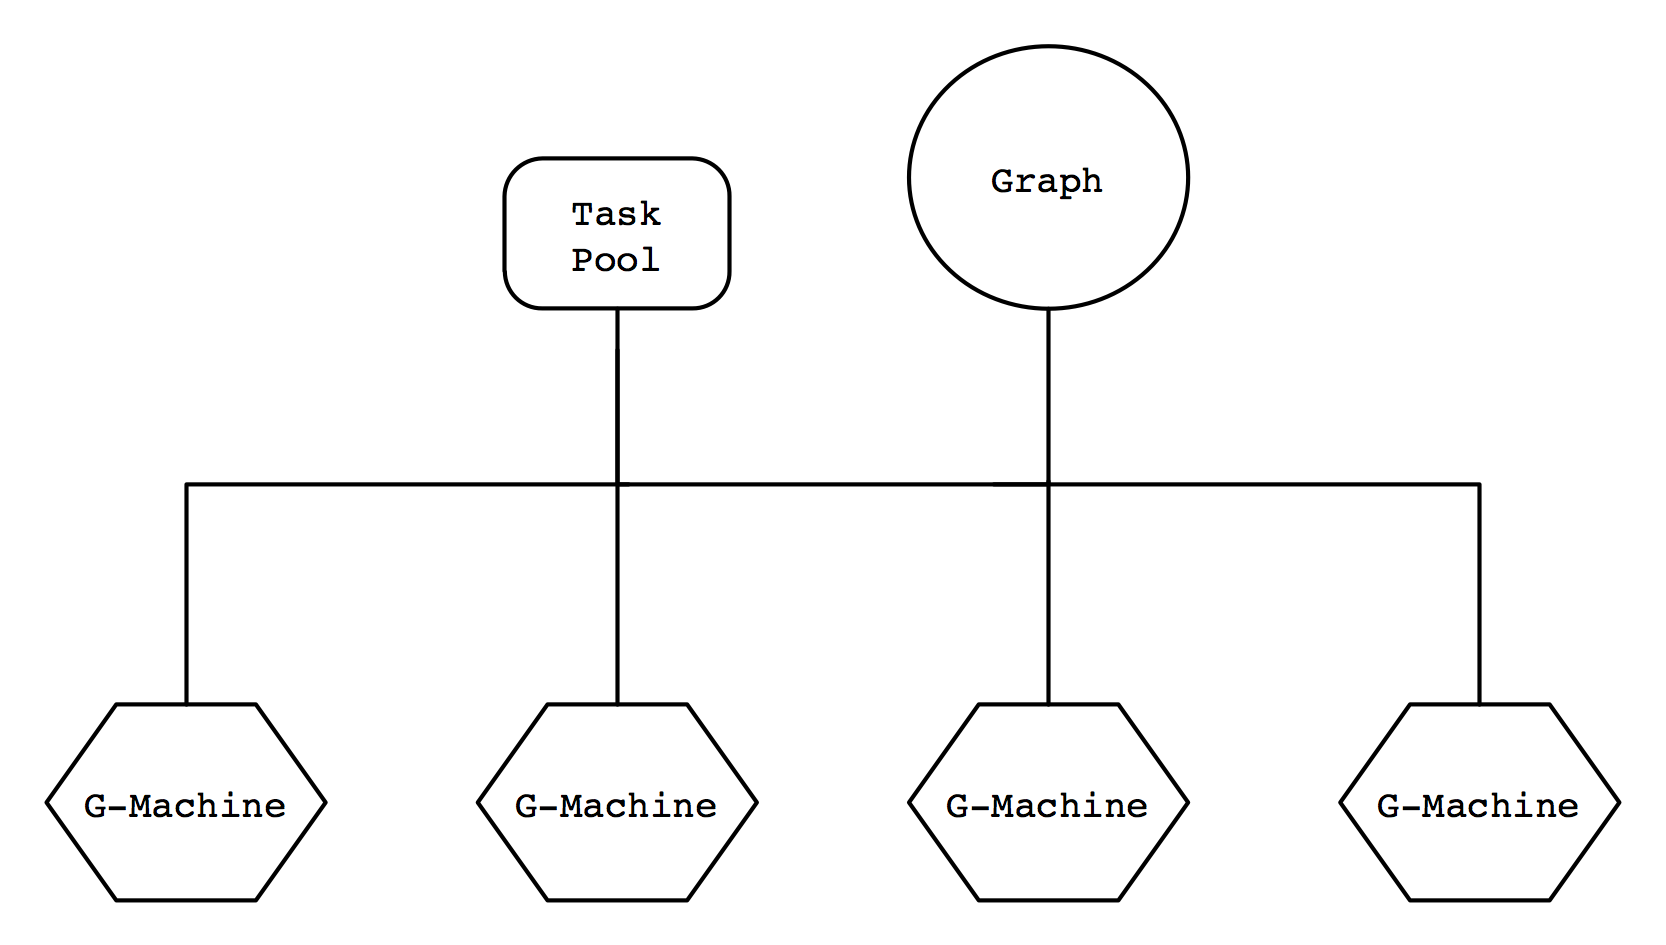
\includegraphics[scale=.3]{figures/simpleParallel.png}
    \end{figure}

\pause
Even this simple strategy has a number of problems to address
\end{frame}

\begin{frame}{$<\nu, G>\-Machine$ \citep{vGMachine}}
\begin{itemize}
    \item
        Like the Parallel G-Machine the $<\nu, G>\-Machine$ stores a central graph and task pool
    \item
\pause
        Unlike the PGM, it is packet based instead of stack based
\end{itemize}
\end{frame}

\begin{frame}{A $<\nu, G>\-Machine$ Packet}

    \begin{figure}
    \centering
        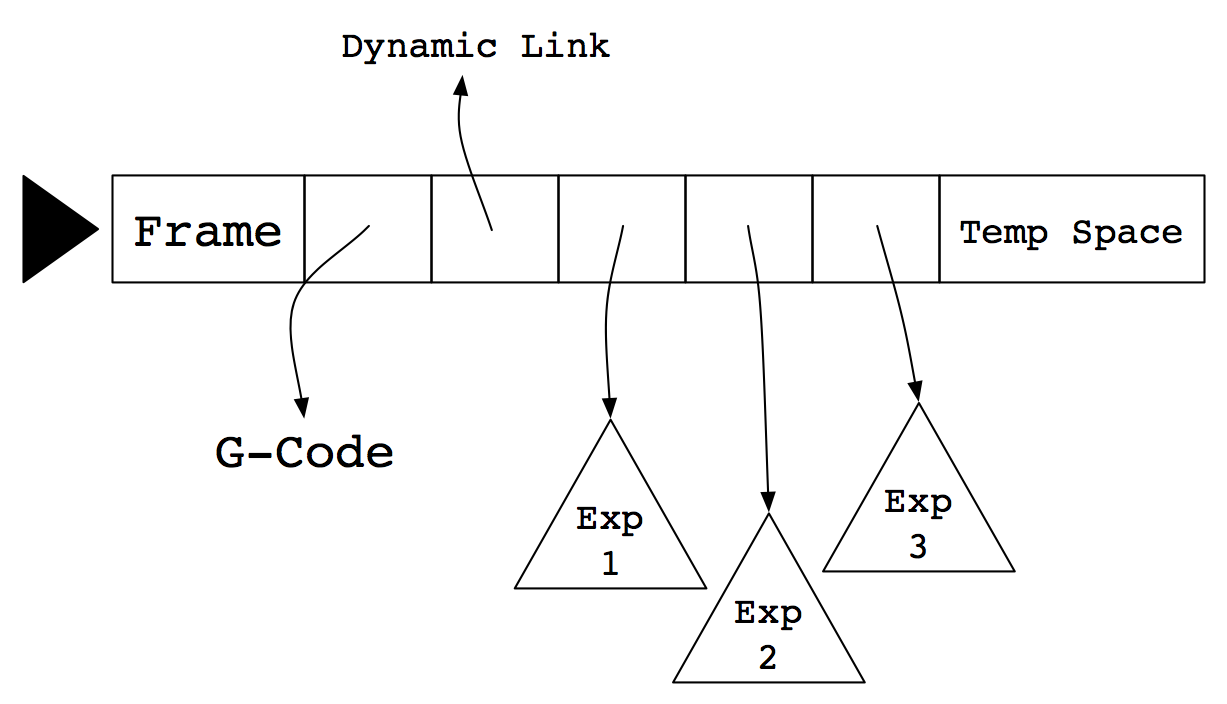
\includegraphics[scale=.3]{figures/packet.png}
        \caption{A $<\nu, G>\-Machine$ packet}
    \end{figure}
\end{frame}

\begin{frame}{A $<\nu, G>\-Machine$ Graph}
    \begin{figure}
    \centering
        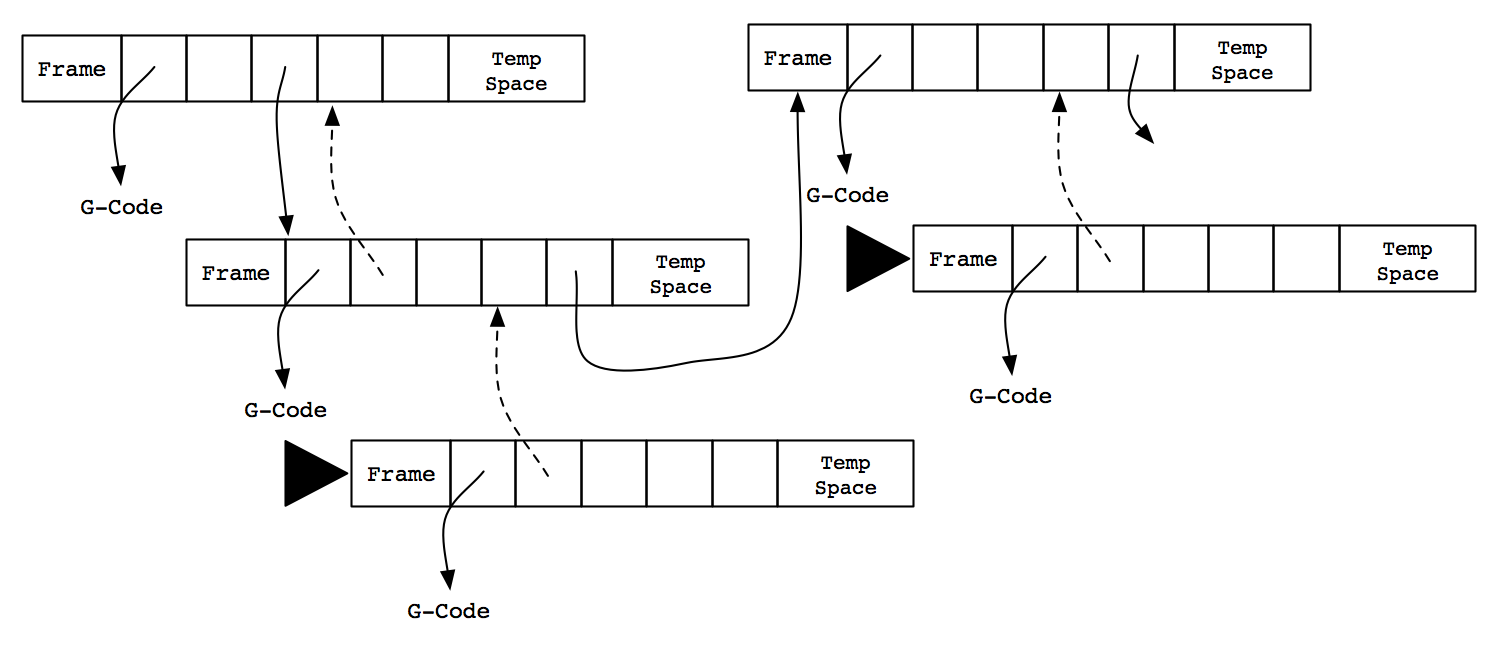
\includegraphics[scale=.4]{figures/vGraph.png}
        \caption{A $<\nu, G>\-Machine$ graph with multiple points of execution}
    \end{figure}
\end{frame}

\subsection[The ABC Machines]{The ABC Machine}
\begin{frame}{Basics}
\begin{quote}
``Basically, the G machine and the ABC machine have much in common, 
although they differ in almost all details.'' -  \citep{dutchBook}
\end{quote}
\pause
The ABC machine was designed as a portable compiler and interpreter \citep{ABCMachine}, with 
this in mind the designers played to the strengths of standard computers. 
\end{frame}

\begin{frame}{Key details of the ABC Machine}
Stack based machine with 3 stacks:
    \begin{enumerate}
        \item The Address stack (A)
        \item The Basic Values Stack (B)
        \item The Control Stack (C)
    \end{enumerate}
\pause
The machine can be thought of as having two parts; the idealized graph rewriting machine 
(The A, B, and the graph), 
and an abstraction from traditional stack based architecture \citep{ABCMachine}.
\end{frame}

\begin{frame}{Details of the Parallel ABC Machine}
\begin{itemize}
    \item Graph is distributed (unlike GM);
\pause
    \item Implements several reducers \emph{per} processor;
\pause
    \item Reducers on the same processor can share a local graph;
\pause
    \item Communication between processors is used for scheduling and the copying of subgraphs.
\end{itemize}
\end{frame}

\section{Physical Machines}

\subsection[GRIP]{GRIP: Graph Reduction In Parallel}
\begin{frame}[fragile]{What GRIP looks like}{}

\begin{figure}[h]
 \centering
 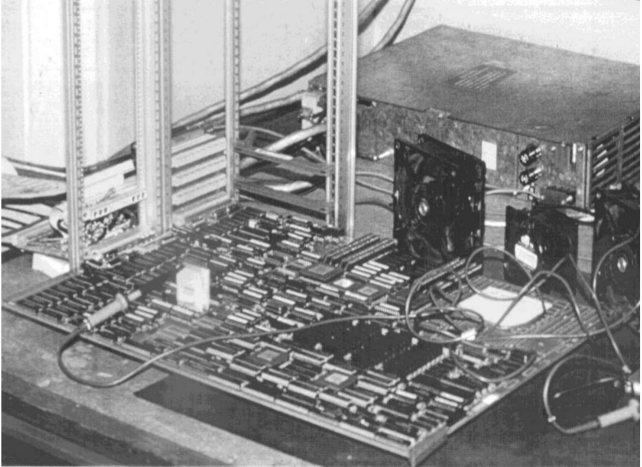
\includegraphics[scale=.4]{figures/GRIP.png}
 \caption{A circuit board for the GRIP machine in the making \citep{PFPAnIntro}}
\end{figure}
\end{frame}

\subsection[ALICE]{ALICE}

\begin{frame}{Quantum Dots as Artificial Atoms}{}
  % - A title should summarize the slide in an understandable fashion
  %   for anyone how does not follow everything on the slide itself.

  Quantum Confinement in 3D -> Artificial atom
  \begin{itemize}
  \item
   Question: What atomic properties are we looking to exploit?
   \pause
  \item
    Answer: Fluorescence.
  \end{itemize}
\end{frame}


\section*{Questions}

\begin{frame}
\centering
Questions
\end{frame}
\begin{frame}[allowframebreaks]{References}  %allowframebreaks

% \sffamily
    \def\bibfont{\scriptsize}
    % \def\bibfont{\footnotesize}
    \bibliography{seminar}

\end{frame} 

\end{document}


